\documentclass[border=2pt]{standalone}
% Shared preamble for the standalone result plots (fig/src/*.tex).
% Compile:  tectonic -X compile fig/src/<name>.tex --outdir fig/src/out
% then copy fig/src/out/<name>.pdf over fig/<name>.pdf
%
% Palette matches the paper: wacvblue is main.tex's link colour, orange is xcolor's.
\usepackage{iftex}
\ifXeTeX
  \usepackage{fontspec}
  \setmainfont{texgyretermes}[Extension=.otf, UprightFont=*-regular,
    BoldFont=*-bold, ItalicFont=*-italic, BoldItalicFont=*-bolditalic]
\fi
\usepackage{pgfplots}
\pgfplotsset{compat=1.18}
\usepackage{amsmath}
\definecolor{wacvblue}{rgb}{0.21,0.49,0.74}
\pgfplotsset{
  resultaxis/.style={
    axis background/.style={fill=white},
    grid=major, ymajorgrids=true, xmajorgrids=false,
    grid style={gray!25, line width=0.3pt},
    tick align=outside, tick pos=left,
    label style={font=\small}, tick label style={font=\small},
    legend style={font=\small, draw=gray!50, fill=white, fill opacity=0.9,
                  text opacity=1, inner sep=2pt},
  },
  vidmark/.style={wacvblue, mark=*, thick, mark size=2.2pt},
  eegmark/.style={orange, mark=o, thick, dashed, mark size=2.2pt},
}

\begin{document}
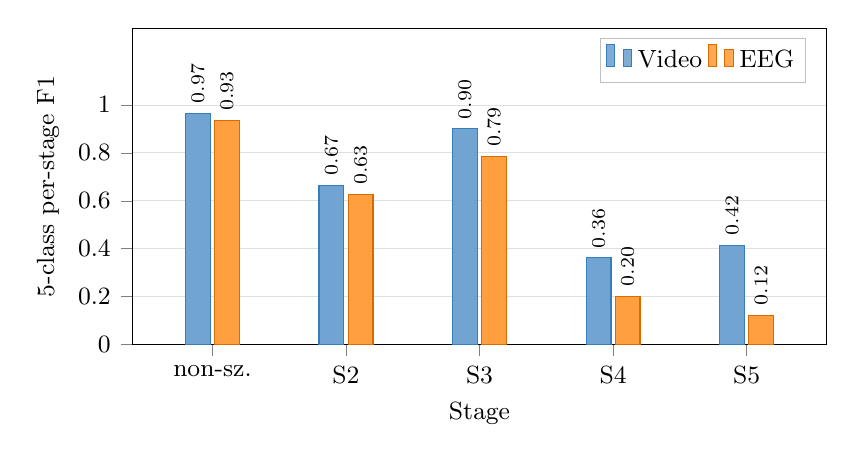
\begin{tikzpicture}
\begin{axis}[
  resultaxis,
  width=10.4cm, height=5.6cm,
  ybar=1.5pt, bar width=9pt,
  xlabel={Stage}, ylabel={5-class per-stage F1},
  symbolic x coords={non-sz., S2, S3, S4, S5},
  xtick=data, xmin={non-sz.}, xmax={S5},
  enlarge x limits=0.15,
  ymin=0, ymax=1.32, ytick={0,0.2,0.4,0.6,0.8,1.0},
  yticklabel style={/pgf/number format/fixed,/pgf/number format/precision=1},
  legend pos=north east, legend columns=2, legend cell align=left,
  nodes near coords, nodes near coords style={rotate=90, anchor=west,
    font=\scriptsize, /pgf/number format/fixed, /pgf/number format/fixed zerofill, /pgf/number format/precision=2},
]
\addplot[draw=wacvblue, fill=wacvblue!70] coordinates
  {(non-sz.,0.966) (S2,0.665) (S3,0.900) (S4,0.362) (S5,0.415)};
\addlegendentry{Video}
\addplot[draw=orange!85!black, fill=orange!75] coordinates
  {(non-sz.,0.934) (S2,0.626) (S3,0.785) (S4,0.202) (S5,0.123)};
\addlegendentry{EEG}
\end{axis}
\end{tikzpicture}
\end{document}
